\subsection{Adding a break time}
In the \emph{Travlendar+} application if the user wants to have some free time he can create a break time. For instance, if the user wants to have lunch at 1 p.m. he can add to his calendar a break time task. This particular kind of task is scheduled according to the user's preferences as a normal task, with flexible time and periodicity but, without a specific location: we suppose that the user will have a break close to where he is.
In addition, if the break time is scheduled close to lunch time, then the \emph{Travlendar+} System will suggest the user a place where to eat.


\begin{table}[H]
	\centering
    
    \begin{tabular}{|p{3.5cm}|p{10.3cm}|}
    
    \hline
    \textbf{\large{Actors}}  			& \tabitem User\\
    
    \hline
    \textbf{\large{Goals}} 				& \ref{goal:task}; \ref{goal:breakTask}; \ref{goal:taskBehavior}; \ref{goal:preferences}; \ref{goal:retakeCar}\\
    
    \hline
    \textbf{\large{Enter Condition}}	& The user should be logged in the                                                        \emph{Travlendar+} system\\
    
    \hline
    \textbf{\large{Events Flow}}		& \begin{enumerate}[leftmargin=0.5cm]
                                          	\item The user presses the "Add a Task" button
                                          	\item The user select "Break Time" as task preferences
                                          	\item The user insert some additional information about the task, such as the time when he wants to do that break
                                          	\item The user select the repetition of that break time task
                                          	\item The user should approve or discard the task
                                          	\item Finally the system compute a schedule according the user's preferences and the break time just inserted
                                          \end{enumerate}
    										\\
    \hline
    \textbf{\large{Exit Condition}} 	& The user either accept the proposed schedule or discard it\\
    
    \hline
    \textbf{\large{Exception}} 			& The break time just inserted is overlapped with other tasks                                         yet inserted in the user's calendar, so the user should                                           select another break time or cancel the other task\\
    
    \hline
    
    
    \end{tabular}
	
\end{table}

\begin{figure}[H]
\centering
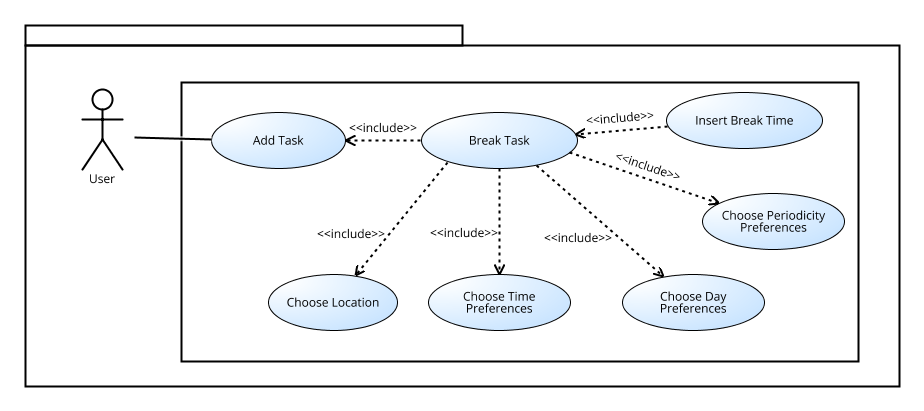
\includegraphics[scale=0.5]{Pictures/UseCaseDiagram/Add_a_break_time.png}
\caption{UML Use Case Diagram for the addition of a break time task }
\end{figure}
